% 第 8 章：设计、制作、调试与结果
\section{设计 制作 调试与结果}

\subsection{项目设计过程}

本项目的设计过程主要经历了方案选型、原理学习、功能验证、整机联调和结构完善五个阶段。项目初期，我们希望通过制作一套实际装置学习磁场定向控制（FOC）算法，最初考虑以平衡车为实现目标。经过资料调研与方案比较后，我们认为智能旋钮能够在较小的硬件规模下直观呈现位置闭环、转矩控制和触觉反馈，更适合作为 FOC 的学习与实践载体，因此最终确定以多功能智能旋钮为项目方向，并参考了 \href{https://github.com/scottbez1/smartknob}{SmartKnob 开源项目}的软件可配置限位与虚拟档位设计思路。

在原理学习与功能验证阶段，我们采购了 DengFOC-V3P 开发板及配套电机套件，结合教学课程学习坐标变换、位置检测、电流控制和闭环调节等 FOC 核心原理。随后在 PlatformIO 环境中逐步完成电机驱动与参数调试，并分别实现连续旋转、档位吸附、限位和回弹等触感效果。通过这一阶段的实践，我们进一步熟悉了 ESP32、磁编码器、电机驱动套件及嵌入式开发工具链的使用方法，也为后续人机交互功能奠定了基础。

进入整机设计阶段后，为满足图形界面显示需求，系统加入了 ST7789 显示屏并采用 LVGL 构建交互页面。由于 DengFOC-V3P 开发板可用引脚数量有限，电机驱动、角度传感器、显示屏和触摸输入还需要分别满足 PWM、I\textsuperscript{2}C、SPI 等接口要求，直接接线不仅繁杂，也不利于稳定调试。为解决这一问题，我们自主设计了转接板，对电源与信号接口进行集中引出和重新分配，并完成焊接、导通检查与上电测试，从而提高了整机连接的可靠性。

硬件基础稳定后，项目进入软硬件联调阶段。我们利用 ESP32 的 FreeRTOS 双核与任务调度能力，将电机控制和 LVGL 图形显示分别组织为独立任务，通过共享状态与消息实现旋钮触感、界面焦点和页面切换之间的协同。完成主界面交互框架后，小组成员分别负责不同功能页面的开发，再统一进行集成、稳定性测试和代码整理。

最后，为提升设备的完整性与外观效果，我们使用 SolidWorks 对 SuperKnob 外壳及内部安装结构进行建模，并结合显示屏、电机、转接板和连接线的实际尺寸反复调整结构。完成零件制作与整机组装后，项目形成了集电机触觉反馈、图形界面和多种应用功能于一体的多功能智能旋钮。

\subsection{硬件制作与整机装配}

\subsubsection{转接板}

本项目的板卡采用 DengFOC-V3P 开发板及其配套电机驱动板。原版 SmartKnob 的 PCB 与元器件以 0402 封装为主，尺寸小、手工焊接难以保证质量，因此我们没有直接复刻其电路板，而是另做一块转接板，把分散的接口按功能集中组织。如图 \ref{fig:adapter} 所示，转接板正面以 8 pin 排母连接显示屏，中部排母插接到驱动板，下方 4 pin 排针排母引出 AS5600 编码器的 I\textsuperscript{2}C 信号，从而把显示屏、驱动板和编码器三条接口统一到一块板上。

\begin{figure}[H]
\centering
\begin{minipage}[b]{0.32\linewidth}
  \centering
  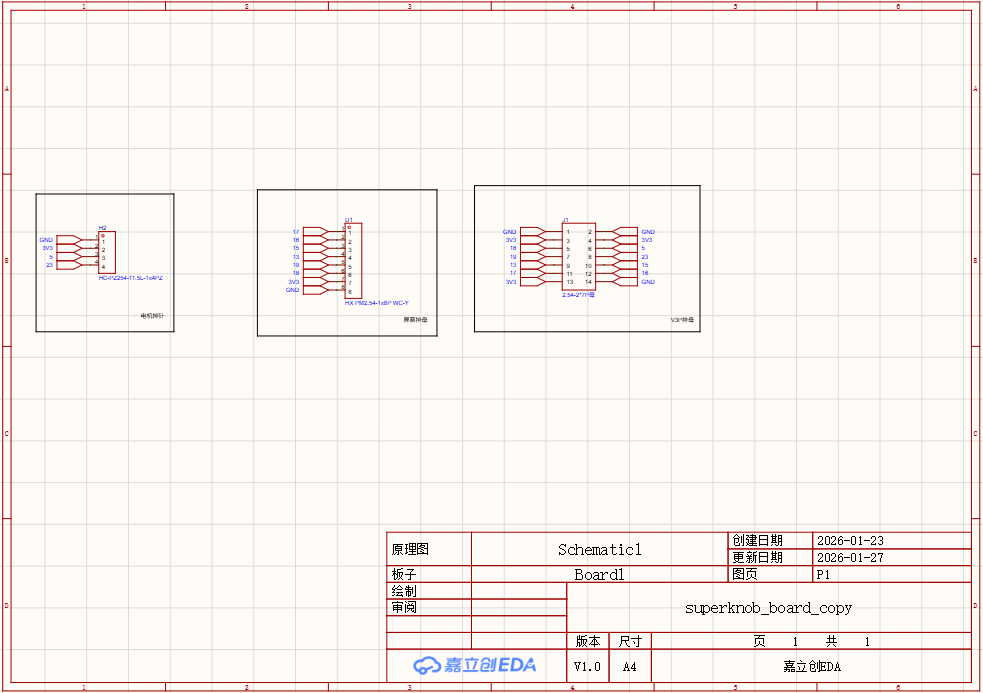
\includegraphics[width=\linewidth]{figures/adapter_display.png}
  \par\small 8 pin 排母接显示屏
\end{minipage}\hfill
\begin{minipage}[b]{0.32\linewidth}
  \centering
  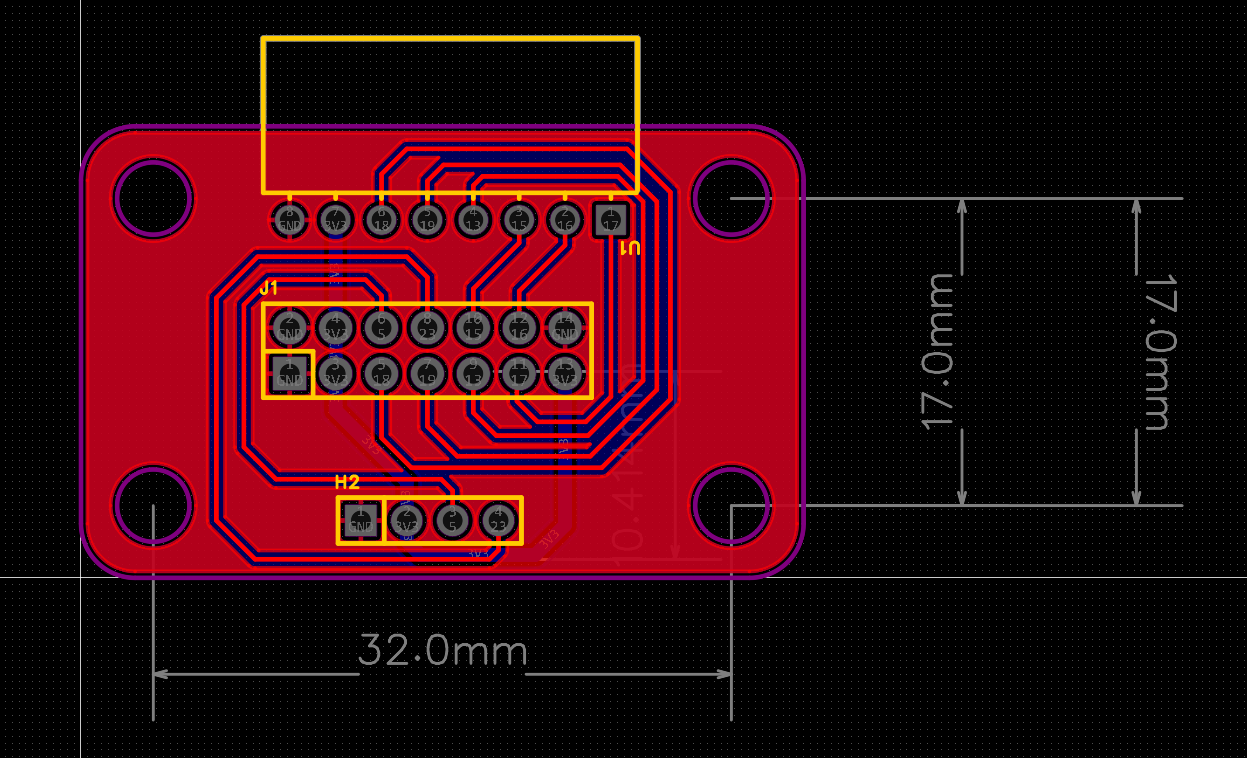
\includegraphics[width=\linewidth]{figures/adapter_driver.png}
  \par\small 排母插接驱动板
\end{minipage}\hfill
\begin{minipage}[b]{0.32\linewidth}
  \centering
  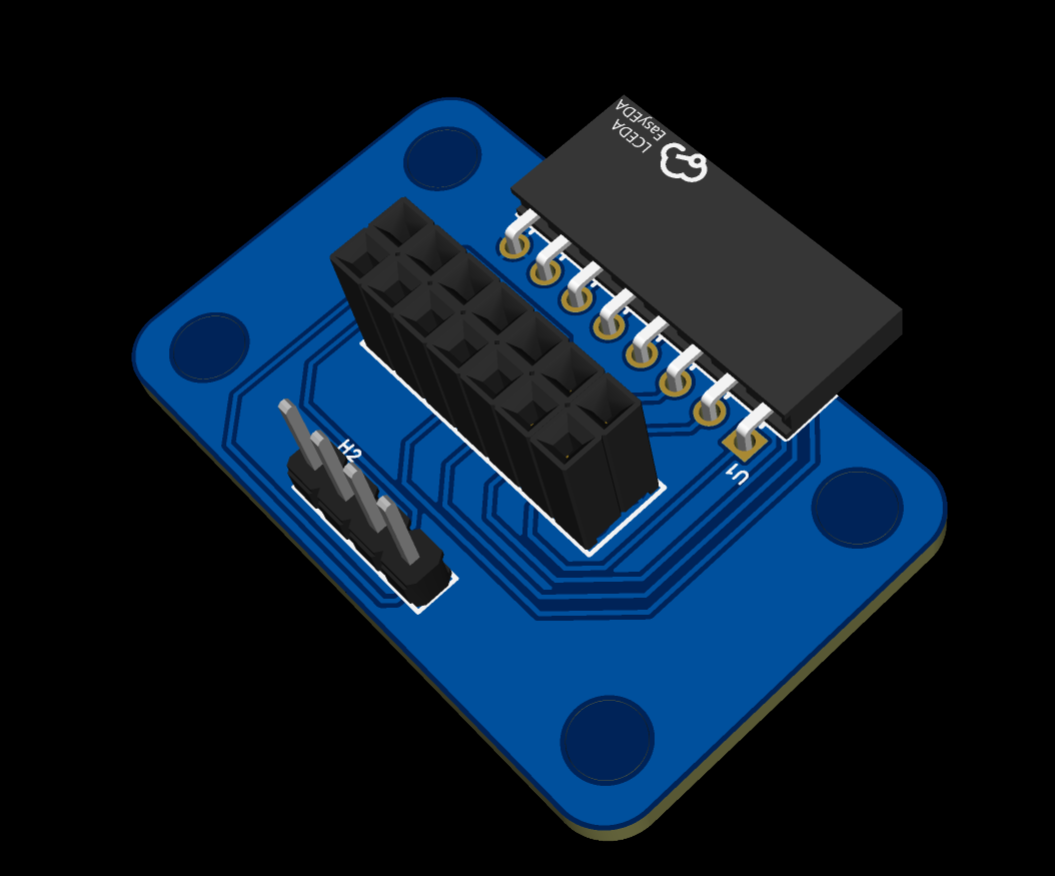
\includegraphics[width=\linewidth]{figures/adapter_encoder.png}
  \par\small 4 pin 排针接编码器 I\textsuperscript{2}C
\end{minipage}
\caption{转接板的显示屏、驱动板与编码器接口}
\label{fig:adapter}
\end{figure}

\subsubsection{外壳建模与装配}

外壳及内部安装结构采用 SolidWorks 建模并以 3D 打印制作，如图 \ref{fig:shell} 所示。建模时按显示屏、电机、转接板、编码器与连接线的实际尺寸确定各安装定位，反复调整以保证结构强度与装配间隙；打印完成后，按磁铁与电机轴同轴、编码器与磁铁间距合适、显示屏固定稳固的要求完成装配。至此，转接板与外壳共同把分散的电气接口和机械零件组织为一个整体，为后续联调提供了稳定可靠的硬件基础。

\begin{figure}[H]
\centering
\begin{minipage}[b]{0.48\linewidth}
  \centering
  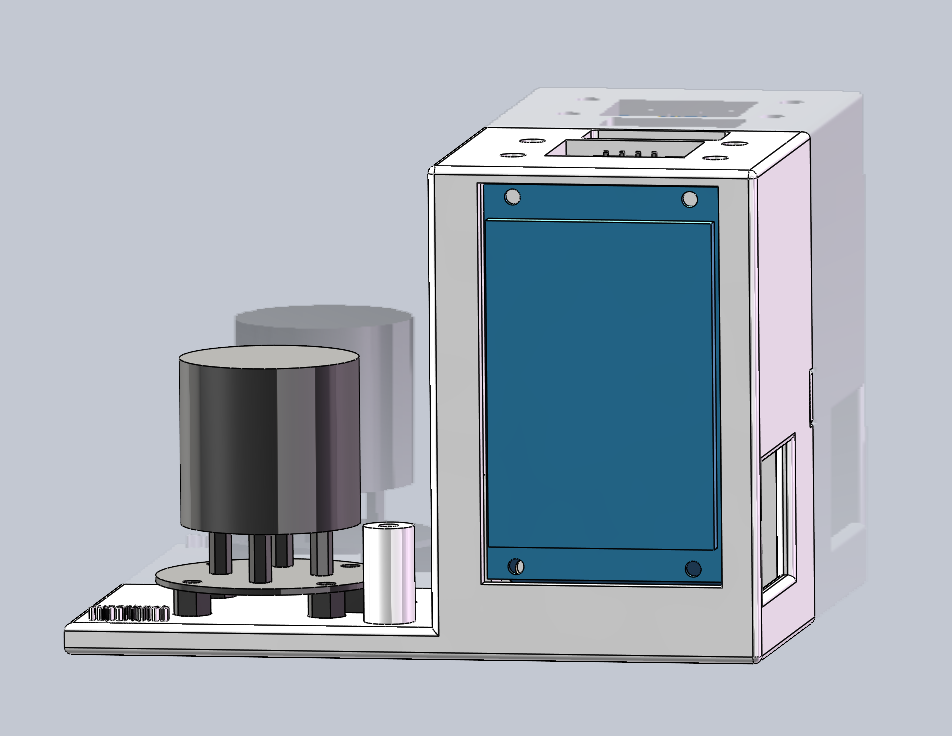
\includegraphics[width=\linewidth]{figures/shell_model_1.png}
\end{minipage}\hfill
\begin{minipage}[b]{0.48\linewidth}
  \centering
  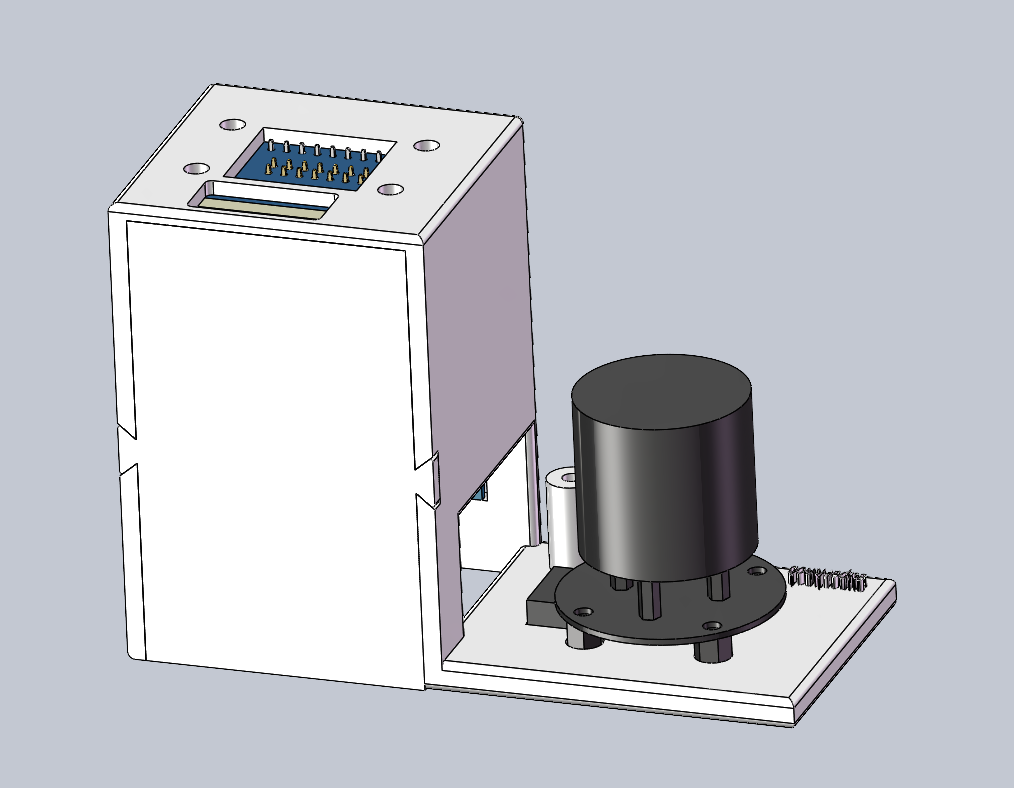
\includegraphics[width=\linewidth]{figures/shell_model_2.png}
\end{minipage}
\caption{SolidWorks 外壳建模}
\label{fig:shell}
\end{figure}

\subsection{软硬件联调过程}

\subsubsection{从编译烧录到屏幕正常显示}

联调开始时，工程还不能稳定完成编译和烧录。我们先在 PlatformIO 中补齐依赖和 LVGL 配置，并解决旧工具链不兼容中文路径的问题。第一次打开串口时输出全是乱码，核对程序后才发现监视器仍使用 9600 baud，而代码设置为 115200 baud；统一波特率后，启动信息终于能够正常阅读。此后每次修改都先确认编译通过，再烧录并查看串口输出，许多问题也因此更容易定位。

屏幕无显示是耗时较长的一次排查。我们先确认背光和供电，再逐项核对屏幕型号、SPI 引脚以及 LVGL 的刷新设置，最后发现实物使用 ST7789，原来的部分配置并不匹配。修改驱动和引脚后，屏幕已经能够点亮，但运行仍不稳定，于是又补充 LVGL 时钟设置，并把显示缓冲改为单个 40 行缓冲，减少内存占用。经过这些调整，页面刷新恢复正常，也为后来加入蓝牙和风扇功能留出了空间。

\subsubsection{触摸、电机与功能页面调试}

触摸键曾出现按一下却连续触发多次的问题。起初我们怀疑 GPIO0 本身受到下载功能影响，尝试把触摸输入改到 GPIO4，但实机现象没有明显改善，因此撤销了这次修改。之后我们改为连续检测到 4 次有效信号才认为按下，并规定手指松开后才能接受下一次输入。电脑控制模式还分别设置按下和松开的阈值，避免数值在临界位置波动。最终单次触摸能够稳定对应一次页面确认或模式切换。

电机不能正常转动时，串口中曾出现 \texttt{Error 263}。查阅并对照运行状态后，我们确认问题来自 AS5600 编码器未被识别，随后重新检查电机独立供电、共地、SDA/SCL 接线和磁铁位置。编码器恢复读数后，再继续调整 FOC 参数和各页面的手感，避免把接线问题误认为控制参数不合适。

风扇功能则按“先读、再写、最后联动页面”的顺序完成。我们先验证 ESP32 能找到风扇并读回型号和状态，再加入开关、风速和左右转动指令。页面接入后发现网络回复会拖慢界面，因此将通信移到单独任务，并合并快速旋转时产生的重复风速请求。随后又处理了中文显示方框、档位到达边界后旋钮难以继续转动等问题。每解决一个问题，都重新烧录并在实机上检查，而不是一次加入全部功能后再集中排错。

表 \ref{tab:debug-loop} 汇总了联调过程中几项较有代表性的问题。

\begin{table}[H]
\centering
\small
\begin{tabular}{p{0.19\linewidth}p{0.26\linewidth}p{0.40\linewidth}}
\toprule
现象 & 定位到的原因 & 处理与验证 \cr
\midrule
工程无法完整链接 & LVGL 配置缺失，旧工具链不兼容中文路径 & 补齐配置并调整工程路径，直到固件能够稳定生成 \cr
屏幕无显示 & 屏幕型号和部分引脚配置与实物不一致 & 改用 ST7789 配置，重新核对 SPI、背光和刷新设置 \cr
触摸重复触发 & 按住时被程序连续识别为多次点击 & 增加连续采样、按下锁定和松开后解锁 \cr
风扇调节时界面卡顿 & 页面需要等待每一次网络回复 & 将联网控制放入单独任务，并合并重复的调速请求 \cr
页面中文显示方框 & 默认字体不包含页面所需汉字 & 根据实际用字重新生成中文字体并检查页面布局 \cr
\bottomrule
\end{tabular}
\caption{主要故障的定位与闭环处理}
\label{tab:debug-loop}
\end{table}

\subsubsection{联调结果}

完成上述调试后，同一套硬件已经能够运行主界面、不同旋钮手感、番茄钟、音乐、两款小游戏、BLE 电脑控制和局域网风扇控制。实机演示中，菜单焦点能随旋钮档位移动，不同页面会切换相应手感；电脑可以收到滚轮、音量、Alt+Tab 和鼠标按键操作，风扇的开关和风速也能随旋钮改变。

项目仍有一些可以继续完善的地方。现有硬件没有相电流采样，手感在负载变化时还不够一致；进入 BLE 模式需要软重启；风扇左右转动的单次角度以及断网后的恢复效果也还需要更多实机测试。这些问题没有影响目前的主要演示，但也让我们认识到，完成页面和控制代码只是第一步，稳定性往往需要在反复烧录、观察和调整中逐渐提高。

